\section{Categoría de homotopías}
En la sección anterior, se termino dando una definición de categoría con
\(\mathscr{Top}_*\) y el functor \(F : \mathscr{Top} \to
\mathscr{Grp}\). Los morfismos en \(\mathscr{Top}_*\) correspondían a
funciones continuas entre espacios topológicos. En particular los
homeomorfismos inducían bajo \(F\) isomorfismos de grupos. Pero hay
espacios que a pesar de no ser homeomorfos poseen el mismo grupo
fundamental y para estos el functor entre \(\mathscr{Top}_* \to
\mathscr{Grp}\) es ciego a su estructura. Esto es insatisfactorio
pensando en la meta original de clasificar diferentes espacio
topológicos y nos hace pensar en que tal vez la noción de homeomorfismos
es mucho mas fuerte de lo que necesitamos.

Entre las nociones alternativas mas populares se encuentra las
\emph{equivalencias homotópicas}. Su popularidad se debe a que son mas
débiles que un homeomorfismo y que corresponden a los morfismos en una
nueva estructura categórica denotada por \(\mathscr{HoTop}_*\), la cual
contiene como sub-categoría a \(\mathscr{Top}_*\) (modulo functor). La
motivación de su construcción es natural a partir del estudio de
retracciones, el cual iniciaremos ahora e iremos generalizando
debidamente.

\subsection{Retracciones}
Previo al estudio tal de las retracción, iniciaremos estudiando un
pequeño lema técnico con respecto a la composición y la función
identidad, ya que este aparecerá repetidamente a lo largo de esta
subseccion.
\begin{lema}
  Sea \(f : X \to Y\) e \(g : Y \to X\) dos funciones. Si \( g \circ f =
  h : X \to X \), con \(h\) una biyeccion, entonces \(f\) es inyectiva y
  \(g\) es sobreyectiva.
\end{lema}
\begin{proof}
  Se argumenta por contradicción. Supongamos que \(f\) no es inyectiva o
  que \(g\) no es sobreyectiva. Tomando el primer caso para \(f\), se
  tiene que existen \(x_1 , x_2 \in X,\ x_1 \neq x_2\) que cumplen
  \[ f (x_1) = f(x_2) \]
  Dado que \(g\) es una función, debe de cumplirse que esta mantiene la igualdad
  \[ g (f (x_1)) = g (f(x_2)) \]
  \[ \iff h (x_1) = h(x_2) \]
  Lo cual es una contradicción con la biyectividad de \(h\).

  Por otro lado, suponiendo que \(g\) no es sobreyectiva, debería de
  existir \(x \in X\) tal que no exista \( y \in Y\) que \(g (y) = x\).
  Pero por hipótesis, el elemento \(f(h^{-1}(x)) \in Y\) es tal que \(g
  (f (h^{-1}(x))) = x\). Mostrando así que \(g\) es en efecto
  sobreyectiva.
\end{proof}
\begin{corolario} \label{thm:comp-identidad}
  Sea \(f : X \to Y\) e \(g : Y \to X\) dos funciones. Si \( g \circ f =
  Id : X \to X \), entonces \(f\) es inyectiva y \(g\) es sobreyectiva.
\end{corolario}
\noindent Ahora procederemos directamente a la definición
de retracción.
\begin{definicion}[Retraccion]
  Sea \(X\) un espacio topológico. El conjunto \(A \subset X\) es una
  retracción de \(X\) si existe un mapeo continuo \(r : X \to A\) tal que
  \[ r \mid_{A} (x) = x \]
  con \(r \mid_{A}\) siendo la restriccion de \(r\) al dominio \(A\). En
  caso de cumplirse esto, \(r\) es llamada la aplicación retracción de
  \(X\) en \(A\).
\end{definicion}
\noindent El nombre de aplicación retracción es intuitivo al ver que es
un mapeo a un subconjunto de un espacio. Toda aplicación retracción
tiene un \emph{dual} que identifica los elementos de un subconjunto con
ellos mismos en el espacio ambiente. Dicha función es llamada aplicación
inclusión; definida formalmente:
\begin{definicion}[Aplicación inclusión]
  Sea \(X\) un espacio topológico y \(A \subset X\) un subconjunto
  arbitrario. La función
  \begin{align*}
     j : A &\longrightarrow X \\
     a &\longmapsto a
  \end{align*}
  es llamada la aplicación inclusión de \(A\) en \(X\).
\end{definicion}
\noindent Las aplicaciones retracción y la inclusión para algún cierta
retracción \(A \subset X\) relacionan los grupos fundamentales de un
espacio \(X\) con el de \(A\) mediante el siguiente teorema.
\begin{teorema} \label{thm:retraccion-inclusion}
Si \(A \subset X\) es una retracción, entonces la aplicación inclusión
\(j : A \to X\) induce un homomorfismo de grupos fundamentales \(j_{*} :
\pi(A, a) \to \pi(X,a)\) inyectivo para todo \(a \in A\).
\end{teorema}
\begin{proof}
  La composición \(r \circ j : A \to A\) es la función identidad de
  \(A\). Tenemos las siguientes igualdades
  \begin{gather*}
    r \circ j \equiv Id \\
    \implies (r \circ j)_* \equiv Id_* \\
    \iff r_* \circ j_* \equiv Id_*
  \end{gather*}
  Por el corolario \ref{thm:comp-identidad}, esto implica que \(r_{*}\)
  es sobreyectiva y que \(j_{*}\) es inyectiva.
\end{proof}
La existencia de una retracción nos da un embedimiento del grupo fundamental de
\( A \) en \(X\) mediante la aplicación inclusión. Ya podemos ver un
poco de las consecuencias de este resultado, por ejemplo diciéndonos
gracias a su contra-positivo que no existe una retracción de \(B^2\) en
\(S^1\).
\begin{gather*}
  S^1 := \{ (x,y) \in \Re^2 \mid x^2 + y^2 = 1 \} \\
  B^2 := \{ (x,y) \in \Re^2 \mid x^2 + y^2 \leq 1 \} \\
\end{gather*}
Ya que si lo hubiera, el homomorfismo inducido por la inclusión \(j_* :
\pi (S^1, a) \to \pi (B^2, a)\) para todo \(a \in S^1\) seria
inyectiva, pero el grupo fundamental de \(B^2\) es trivial (es un
conjunto convexo) y el de \(S^1\) no lo es (corresponde a \((\mathbb Z,
+)\)); esto ultimo es un resultado que veremos mas adelante mediante
espacios cubrimientos.

El teorema \ref{thm:retraccion-inclusion} tambien nos permite demostrar
parte lo que habíamos mostrado intuitivamente en la sección
\ref{ex:R2-11} respecto el grupo fundamental de \(\Re ^2 \backslash
\{(1,1)\}\).
\begin{corolario} \label{cor:retraccion-R2-S1-inyectivo}
  Para todo \(\vec a \in \Re ^2\), el grupo fundamental de \(\Re ^2
\backslash \{\vec a\}\) contiene a un subgrupo isomorfo a \((\mathbb Z, +)\).
\end{corolario}
\begin{proof}
Dado que para todo \(\vec a \in \Re ^2 \), siempre existe
el homeomorfismo
\begin{align*}
   f_a : \Re^2 \backslash \{\vec a\} &\longrightarrow \Re ^2 \backslash
      \{\vec 0\} \\
   \vec x &\longmapsto \vec x - \vec a
\end{align*}
Por tanto podemos estudiar el grupo fundamental de \(\Re ^2 - \{\vec
0\}\) sin perdida de generalidad mediante el teorema
\ref{thm:homoemorfismo-isomorfismo}.

Para este, podemos construir la siguiente aplicación retracción a
\(S^1\)
\begin{align*}
   r : \Re ^2 \backslash \{\vec 0\} &\longrightarrow S^1 \\
   x &\longmapsto \frac x {\lVert x \rVert}
\end{align*}
Esta cumple la condición de continuidad trivialmente y dado que todo
elemento de \(S^1\) posee norma \(1\), para estos es la identidad
como es requerido para una retracción. Luego, por teorema
\ref{thm:retraccion-inclusion} tenemos la existencia un homomorfismo
inducido
\[ j_* : \pi (S^1 , y_0) \to \pi (\Re ^2 \backslash \{\vec a\}, y_0) \]
inyectivo de grupos fundamentales para todo \(y_0 \in S^1 \). El
grupo fundamental de \(\left( \pi (S^1, y_0) , * \right) \) es \( (\mathbb Z, +)\)
por el teorema \ref{thm:grupo-S1} a presentarse posteriormente.
Mostramos asi que hay un subgrupo de \(\left( \pi (S^1, y_0), * \right)
\) isomorfo a \((Z,+)\).
\end{proof}

Si mediante algún resultado pudiéramos probar que \(j_{*}\) es además
sobreyectiva tendríamos listo nuestro isomorfismo de grupos. Esto es
posible de construir, pero para eso necesitamos algunos resultados
técnicos previos.

\begin{lema} \label{lem:homotopic-inducing}
  Sean \(h,k : (X, x_0) \to (Y, y_0)\) dos mapeos continuos. Si \(h\) y
  \(k\) son homotopicos y si la imagen de \(x_0\) bajo esta homotopía permanece
  fija en \(y_0\), entonces \(h_*\) e \(k_*\) son iguales.
\end{lema}
% TODO: hay que ser mas preciso porque debemos mantener la homotopía
% fija en un punto. Hay que hacer enfasis en el grupo fundamental
% basandose en lo fijo de dicho punto.
\begin{proof}
  Queremos mostrar que \(\forall [f] \in \pi (X,x_0)\), se cumple que
  \(h_* ([f]) = k_* ([f])\). Esto equivale a mostrar que
  \[ [h \circ f] = [k \circ f] \]
  Es decir, debemos de encontrar una arco homotopía entre \((h \circ
  f)\) e \( (k \circ f)\).

  Para esto, usamos la homotopía entre \(h\) y \(k\) dada por la hipótesis
  \[H : X \times I \to Y \]
  Además, notamos que el representante de clase \(f\) es una función \(f
  : I \to X\) . Con ella, podemos construir una homotopía \(M : I \times I
  \to Y \) pre-componiendo como
  \[ M(z, t) \coloneqq H \circ (f(z), t) \]
  La cual es una homotopía entre \((h \circ f)\) e \((k \circ f)\)

  La importancia de que se cumpla que \( \forall t \in I,\ M (x_0, t) =
  y_0\) es para que cumpla la segunda ecuación de la definición
  \ref{def:arco-homotopia} de arco homotopía. Es decir
  \[ \forall t \in I ,\ M(0,t) = H \left( f (0), t \right) = H (x_0, t)
    = y_0 = H \left( f(1) , t \right) = M (1, t) \]
\end{proof}
\begin{teorema} \label{thm:comp-identidad-homotopia}
  Sea \(f : X \to Y\) y \(g : Y \to X\) funciones continuas. Si \(f
  \circ g\) es homotopico a la identidad \( \mathrm{Id} : Y \to Y\) y
  existe \(y_0 \in Y\) tal que \( (f \circ g ) (y_0) = y_0 \) entonces
  \(f_*\) es sobreyectiva y \(g_*\) es inyectivo.
\end{teorema}
\begin{proof}
  Siendo \(y_0 \in Y\) el punto fijo entre la homotopía de \(f \circ g\)
  y \(\mathrm{Id}\), podemos aplicar sobre estos el lema
  \ref{lem:homotopic-inducing}. Obtenemos así la igualdad
  \[ (f \circ g)_{*} = f_* \circ g_* = \mathrm{Id}_* \]
  Con \(\mathrm{Id}_* : \pi (Y, y_0) \to \pi (Y, y_0)\). Luego
  aplicando el corolario \ref{thm:comp-identidad} sobre esta ecuación
  obtenemos que \(f_*\) es sobreyectiva y que \(g_*\) es inyectiva.
\end{proof}

Esta es exactamente la misma demostración que en el teorema
\ref{thm:comp-identidad}, pero haciendo énfasis lo que significa ser
inyectivo o sobreyectivo en clases de equivalencias. Resulta que ya
tenemos todos los resultados necesarios para expandir el resultado del
corolario \ref{cor:retraccion-R2-S1-inyectivo} sobre la
retracción \(\Re ^2 \backslash \{0\}\) en \(S^1\).

\begin{teorema}
  Para todo \(a \in S^1\), el monomorfismo \(j_* : \pi (S^1, a)
  \to \pi (\Re ^2 - \{0\}, a)\) es un isomorfismo de grupos
  fundamentales.
\end{teorema}
\begin{proof}
  Ya habíamos dicho anteriormente en el corolario
  \ref{cor:retraccion-R2-S1-inyectivo} que \( j_* : \pi (S^1, a) \to \pi
  (\Re ^2 - \{0\}, a)\) es inyectiva como homomorfismo de grupos
  fundamentales, puesto la existencia de la retracción
  \begin{align*}
    r : \Re ^2 \backslash \{0\} &\longrightarrow S^1 \\
    x &\longmapsto \frac x {\lVert x \rVert}
  \end{align*}
  implica por corolario \ref{thm:comp-identidad} la inyectividad de
  \(j_*\).

  Para probar la sobreyectividad de \(j_*\), tomemos la composición
  \[ j \circ r : \Re ^2 \backslash \{0\} \longrightarrow \Re ^2
      \backslash \{0\} \]
    Esta composición \emph{no} es la identidad de \(\Re ^2 \backslash \{0\}
  \) pero es homotópica a esta mediante la homotopía de linea recta
  \[
    H(x,t) := t \cdot x + (1 - t) \cdot \frac x {\lVert x \rVert}
  \]
  Debemos de mostrar que es una homotopía valida en cuanto no cae fuera
  del recorrido. En esta ocasión, no tenemos la hipótesis de recorrido
  convexo sobre la identidad y \(j \circ r\) pues estos son \(\Re ^2
  \backslash \{\vec 0\}\) y \(B[0,1] \backslash \{\vec 0\}\)
  respectivamente. Aun así, esta homotopía es continua solo por ser
  combinación lineal de funciones continuas. Para ver que tiene el
  recorrido correcto, mostraremos \(\vec 0\) no pertenece a la imagen de
  \(H\). Notamos que para todo \(\vec x \in \Re ^2 \backslash \{\vec
  0\}\), se tiene que \(\vec x \) y \( \vec x / \lVert x \rVert\) están en
  el mismo cuadrante y por tanto no existe combinación convexa que resulte
  en \(\vec 0\).

  Notamos también que esta homotopía deja fijo al punto \((1,0)\), luego
  tenemos las hipótesis del teorema \ref{thm:comp-identidad-homotopia} y
  obtenemos que \(j_*\) es además sobreyectiva. Concluimos que \(j_*\) es
  un isomorfismo de grupos fundamentales.
\end{proof}

\subsection{Tipos homotopicos}
Ahora que ya conocemos el esquema de trabajo, podemos generalizar para
espacios que no necesariamente sean retracciones entre si, pero que
posean un par de funciones cuyas composiciones sean homotópicas a la
identidad correspondiente.
\begin{definicion}[Equivalencias homotopicas] \label{def:equivalencias-hom}
  Sean \(f : X \to Y\) e \(g : Y \to X\) mapeos continuos. Supongamos
  que \( g \circ f : X \to X \) es homotopico al mapeo identidad de
  \(X\) y \( f \circ g : Y \to Y \) es homotopico al mapeo identidad de
  \(Y\). Entonces \(f\) y \(g\) son llamadas \emph{equivalencias
  homotopicas} y cada una es una \emph{inversa homotopica} de la otra.
  Si dos espacios poseen un par de equivalencias homotopicas entre ellos,
  se dicen que ambos espacios son del mismo \emph{tipo homotopico}.
\end{definicion}
Podemos ver que en sección anterior, la retracción y la inclusión
correspondían a par de equivalencias homotopicas. Podría pensarse que la
existencia de un par de equivalencias homotopicas entre espacios seria
suficiente para afirmar que poseen el mismo grupo fundamental, esto es
cierto en medida que se sea cuidadoso con los puntos de partida. Este
problema no se manifestaba en retracciones porque el punto de partida se
mantenía fijo en la inclusión. Para ver el problema mas claro,
supongamos que tenemos dos espacios \(X, Y\) junto con un par
equivalencias homotopicas
\[ f : X \to Y \quad g : Y \to X \]
Por hipótesis tenemos que \(g \circ f \simeq Id : X \to X\), pero eso
\textbf{no} nos asegura la existencia de un punto \(x_0 \in X\) que sea
fijo bajo la homotopía entre \( g \circ f\) y \(Id\). Por tanto no
podemos aplicar el lema \ref{lem:homotopic-inducing} pues no podemos
cumplir una de las hipótesis. Resulta que esto es subsanable utilizando
el siguiente lema técnico.

\begin{lema} \label{lem:equiv-hom-lift}
  Sean \(h,k : X \to Y\) mapeos continuos, sea \(h (x_0) = y_0,\ k(x_0)
  = y_1\). Si \(h\) y \(k\) son homotopicos mediante \(H : X \times I
  \to Y\), entonces existe un arco \(\alpha\) en \(Y\) de \(y_0\) a
  \(y_1\) tal que
  \[k_* = \hat \alpha \circ h_* \]
  con \(\hat \alpha\) el conjugado de \(\alpha\) dado por la definicion
  \ref{def:conjugada}. Mas aun, este arco esta dado por la ecuación
  \(\alpha (t) = H (x_0, t)\).
\end{lema}
\begin{proof}
  Hemos de probar que \(\forall [f] \in \pi (X, x_0)\) se cumple que
  \[ k_* ([f]) = \hat \alpha \circ h_* ([f]) \]
  \[ [k \circ f] = [ \alpha^{-1} ] *  [h \circ f] * [\alpha] \]
  \[ [ \alpha ] * [k \circ f] =  [h \circ f] * [\alpha] \]
  Es decir, hemos de construir una homotopía entre estos dos
  representantes de clase. Sea \(H : X \times I \to Y\) la homotopía
  entre \(h\) y \(k\) dada por hipótesis, entonces podemos reescribir
  las funciones de la ultima ecuación definiendo nuevas curvas sobre \(I
  \times I\)
  \[ f_0(t) := \left( f(t), 0 \right), \quad H \circ f_0 = h \circ f \]
  \[ f_1(t) := \left( f(t), 1 \right), \quad H \circ f_1 = k \circ f \]
  \[ c(t) := (x_0, t), \quad H \circ c = \alpha \]

  De igual manera re-definiremos las tres nuevas curvas en términos de
  \(F : I \times I \to X \times I\) dada por la ecuación \(F(s,t) =
  (f(s),t)\). Para esto debemos considerar los cuatro bordes de
  \(I \times I\).
  \[ \beta_0(s) = (s, 0) \quad \beta_1(s) = (s, 1)\]
  \[ \gamma_0(t) = (0, t) \quad \gamma_1(t) = (1, t)\]
  Mostrándose las siguientes igualdades
  \[ F \circ \beta_0 = f_0 \quad F \circ \beta_1 = f_1\]
  \[ F \circ \gamma_0 = c = F \circ \gamma_1 \]

  Notese que los caminos \(\beta_0 * \gamma_1\) y \(\gamma_0 * \beta_1\)
  son los caminos inferior derecho y izquierdo superior del cuadrilátero
  \(I \times I\). Dada la convexidad de este espacio, existe una
  homotopía denotada por \(G : I \times I \to I \times I \) entre ellos.
  Luego por composición \(F \circ G\) es una homotopía entre \(f_0 * c\) y
  \(c * f_1\) y la composición \(H \circ F \circ G\) es una homotopía en
  \(Y\) tal que
  \[ (H \circ f_0) * (H \circ c) = (h \circ f) * \alpha \]
  \[ (H \circ c) * (H \circ f_1) = \alpha * (k \circ f) \]
  Obteniendo así la homotopía buscada.
\end{proof}

La importancia de encontrar dicho arco \(\alpha : I \to Y\) entre los
dos levantamientos proviene del siguiente lema.
%% todo(slack): revisar si este lema es necesario en vista del teorema 2.
\begin{lema} \label{lem:hat-alpha-iso}
\(\hat \alpha : \pi (Y, y_0) \to \pi (Y, y_1)\) es un isomorfismo de
grupos fundamentales.
\end{lema}
\begin{proof}
  Por definición \(\hat \alpha\) es claramente un homomorfismo. Para ver
  que es inyectiva, supongamos que tomamos \([f],[g] \in \pi (Y, y_0),\
  [f] \neq [g]\) tal que se cumple \(\hat \alpha ([f]) = \hat \alpha
  ([g])\). Esto implicaría por reducción que
  \[ [\alpha^{-1}] * [f] * [\alpha] = [\alpha^{-1}] * [g] * [\alpha] \]
  \[ [f] * [\alpha] = [g] * [\alpha] \]
  \[ [f] = [g] \]
  Lo cual es una contradicción

  Para ver la sobreyectividad, para todo elemento \([h]
  \in \pi (Y,y_0)\) existe \( [\alpha] * [h] * [\alpha^{-1}] \in \pi
  (Y,y_0)\) tal que
  \[ \hat \alpha ([\alpha] * [h] * [\alpha^{-1}]) = [h]\]
\end{proof}
Con esto en mente, es fácil ver que se tiene el siguiente corolario
\begin{corolario}
  Sean \(h,k : X \to Y\) dos funciones relacionadas homotopicamente
  tales que \(h (x_0) = y_0\) y \(k(x_0) = y_1\). Si \(h_*\) es inyectiva
  o sobreyectiva o trivial, entonces \(k_*\) también lo es.
\end{corolario}
\begin{proof}
  Dado que por el lema \ref{lem:equiv-hom-lift} tenemos la siguiente
  ecuación entre levantamientos
  \[ k_* = \hat \alpha \circ h_* \]
  Por el lema \ref{lem:hat-alpha-iso} sabemos que \(\hat \alpha\) es
  biyectivo. Por tanto la composición de \(h_*\) inyectiva con \(\hat
  \alpha\) biyectiva es inyectiva. De igual manera para la
  sobreyectividad.
\end{proof}
Con esto podemos al fin plantear que todo par de espacios en el mismo
tipo homotopico poseen el mismo grupo fundamental. Esto gracias a que
podemos evitar la condición de punto fijo en el lema
\ref{lem:homotopic-inducing} gracias a la biyeccion de \(\hat \alpha\).

\begin{teorema}
  Sean \(f : X \to Y\) continua y \(f (x_0) = y_0\). Si existe \(g : Y
  \to X\) tal que \(f\) y \(g\) son una equivalencia homotopica, entonces
  \[ f_* : \pi (X, x_0) \to \pi (Y, y_0)\]
  es un isomorfismo de grupos fundamentales.
\end{teorema}
\noindent Para este teorema, es necesario que seamos un poco mas
específicos con la notacion de levantamientos. Un levantamiento de \(f :
X \to Y\) con respecto a \(x_0\) corresponde a la función
\[ (f_{x_0})_{*} : \pi (X , x_0) \to \pi (Y, y_0)\]
donde \(f(x_0) = y_0\). Ahora podemos proceder con la demostracion.
\begin{proof}
  Fijemos los puntos \(x_1 = g(y_0)\) y \(y_1 = f(x_1)\). Véase que dado
  los diferentes puntos bases se tienen dos homomorfismos inducidos de
  \(f\) con distintos puntos relativos
  \[(f_{x_0})_* : \pi (X, x_0) \to \pi (Y, y_0)\]
  \[(f_{x_1})_* : \pi (X, x_1) \to \pi (Y, y_1)\]
  Además fijaremos que la identificación de \(g_*\) corresponda a
  \[ g_* : \pi (Y, y_0) \to (X, x_1) \]

  Por hipótesis, \(g \circ f : (X, x_0) \to (X, x_1)\) es homotópico a
  la función identidad \(Id : X \to X\). Luego por el lema
  \ref{lem:equiv-hom-lift} se tiene la existencia de un \(\hat \alpha\)
  tal que cumpla la ecuación
  \begin{equation} \label{eq:alpha-f-g}
  g_* \circ (f_{x_0})_* = (g \circ f)_* = \hat \alpha \circ (Id_X)_*
    = \hat \alpha
  \end{equation}
  Por tanto \(g_* \circ (f_{x_0})_*\) es un isomorfismo y esto obliga a
  que \(g_*\) sea sobreyectiva.

  De igual manera, aplicando el análisis anterior a \(f \circ g : \pi
  (Y, y_0) \to (Y, y_1)\) homotópico a la identidad de \(Y\), se
  obtiene que \((f_{x_1})_* \circ g_*\) es un isomorfismo y por tanto
  \(g_*\) es inyectivo también.

  Conociendo la biyectividad de \(g_*\), nos permite pre-componer por su
  inversa \((g_*)^{-1}\) en la ecuación \eqref{eq:alpha-f-g}, obteniendo
  \[ (f_{x_0})_* = (g_*)^{-1} \circ \hat \alpha\]
  luego, la composición de biyeccion es biyeccion y por tanto
  \((f_{x_0})_*\) es un isomorfismo de grupos fundamentales.
\end{proof}

Con estos resultados podemos ver el siguiente ejemplo
\begin{corolario} \label{ex:mobius}
  Sea \(M\) la banda de \emph{Mobius} finita definida por la identificacion
  \[ M := [0,1] \times [0,1] / \sim, \quad (0,y) \sim (1, 1 - y) \]
  Este espacio posee el mismo grupo fundamental de \(S^1\)
\end{corolario}
\begin{proof}
  %%TODO: diagama de M
  Podemos pensar en la banda de \emph{Mobius} como un cuadrado con los
  lados izquierdos y derechos identificados en sentido inverso.
  Definimos la ``banda central'' de este como el conjunto
  \[ D := [0,1] \times \{1 / 2\} / (0, 1 / 2) \sim (1,1 / 2) \]
  (esta identificacion equivale a la de \(M\) para \(y = 1/2\)). Podemos
  definir la siguiente retraccion e inclusion
  \[
    \begin{matrix}
      r : M \to D & j : D \to M \\
      [(x,y)] \mapsto [(x, 1/2)] & x \mapsto x
    \end{matrix}
  \]
  Hemos de probar que \(j \circ r\) es homotopico a la identidad \(Id
  : M \to M\). Definamos la homotopía
  \[ F : M \times I \to M \]
  \[ ([(x,y)], t) \mapsto [(x, \frac t 2 + (1-t) y)] \]
  La cual es claramente continua y cumple que
  \[ x \to F(x,0) \equiv Id,\quad x \to F(x,1) \equiv j \circ r\]
  Luego por teoremas anterior, el grupo fundamental de
  \(M\) es igual al de \(D\).

  La pregunta ahora es ver quien es el grupo fundamental de \(D\).
  Podemos ver que este conjunto es una recta con los dos extremos
  identificados, lo cual luce similar a \(S^1\). Estos espacios son
  homeomorfos mediantes la aplicacion
  \[[(x, 1/2)] \mapsto \exp (2 \pi x)\]
  mostrando asi el resultado deseado.
\end{proof}

\subsection{La categoria \(\mathscr{HoTop}_*\)}
\begin{definicion}
  La categoria \(\mathscr{HoTop}_*\) corresponde a una tripleta
  \((\mathbf{Obj},\mathbf {Mor}, (\hat \circ))\) donde
  \begin{itemize}
  \item \(\mathbf {Obj}\) corresponde a espacio topologicos puntuados de la
    forma \((X, x_0)\).
  \item \(\mathbf {Mor}\) corresponde a un conjunto
    \[ \mathbf{Mor} = \{ [f] \mid f : (X,x_0) \to (Y,y_0),\
      (X,x_0),(Y,y_0) \in \mathbf {Obj} \}\]
    de clases equivalencias homotopicas entre funciones continuas.
  \item \((\hat \circ)\) corresponde a la composición de clases de
    equivalencias tal que si \([f] , [g] \in \mathbf {Mor} \) con
    \[ f : (X,x_0) \to (Y, y_0)\]
    \[ g : (Y, y_0) \to (Z, z_0)\]
    entonces \([g] \, \hat \circ \, [f] := [ g \circ f ] \) es una clase
    de equivalencia de funciones \((X, x_0) \to (Z, z_0)\).
  \end{itemize}
\end{definicion}
Esta categoría tiene los mismos objetos que \(\mathscr{Top}_*\), pero es
diferente en sus morfismos y operador composicion. Es posible ver a
\(\mathscr{Top}_*\) representada por una sub-categoria\footnote{Mismos
objetos pero un subconjunto de los morfismos} de \(\mathscr{HoTop}_*\)
mediante el siguiente functor
\begin{align*}
  G : \mathscr{Top}_* &\longrightarrow \mathscr{HoTop}_* \\
  \left( X , x_0 \right) &\longmapsto \left( X , x_0 \right), \quad
     \left( X, x_0 \right) \in \mathbf {Obj} \left( \mathscr{Top}_* \right) \\
  f &\longmapsto [f], \quad f \in \mathbf {Mor} \left( \mathscr{Top}_* \right)
\end{align*}
pues esta preserva la composicion de categoria de origen en la de
llegada. Ya que por definicion \(\forall f,g \in \mathbf {Mor}
(\mathscr{Top}_*)\) tal que \(f \circ g \in \mathbf {Mor}
(\mathscr{Top}_*)\)
\[ F(f \circ g) = [f \circ g] = [f] \, \hat \circ \, [g] = F(f) \, \hat
\circ \, F(g) \]

En \(\mathscr{Top}_*\) al tomar los morfismos era homeomorfismos,
estaban claramente delimitados los espacios topológicos que tendrían el
mismo grupo fundamental. Pero era posible que hubieran dos familias de
objetos disjuntas en \(\mathscr{Top}_*\) que tuvieran el mismo grupo
fundamental. En \(\mathscr{HoTop}_*\) los espacios homeomorfos tienen
trivialmente un par de equivalencias homotópicas, pero hay estrictamente
menos familias disjuntas en esta categoría, pues como vimos en el
ejemplo \ref{ex:mobius}, a pesar de la banda de Mobius y \(S^1\) no son
homeomorfos (de hecho la banda de Mobius es homeomorfa a un cociente de
\(S^1 \times [-1, 1]\)) poseen el mismo grupo fundamental. Por tanto las
familias de objetos disjuntas con el mismo grupo fundamental son mas
raras en \(\mathscr{HoTop}_*\).

Ahora nos enfocaremos en la estructura categórica, pues esta nos ayudara
a visualizar grupos fundamentales de espacios complejos en base a
espacios mas simples. Una de las herramientas para esto sera el estudio
de los productos y co-productos categóricos.

\begin{definicion}[Producto]
  Sea \(P , X , Y \in \mathbf {Obj}\) objetos arbitrarios de un categoría
  tal que existan \(\pi_x : P \to X,\ \pi_y : P \to Y\) dos morfismos en
  \(\mathbf {Mor}\). Si para todo objeto \(M \in \mathbf {Obj}\) que
  posea morfismos \( f : M \to X,\ g : M \to Y\), existe un morfismo
  \(\theta : M \to P\) en \(\mathbf{Mor}\) tal que se cumplen las
  siguientes ecuaciones
  \[ f = \pi_x \circ \theta, \quad g = \pi_y \circ \theta \]
  entonces \(P\) es un producto de \(X\) e \(Y\).
\end{definicion}
\begin{acotacion}
  La propiedad que debe cumplir el producto \(P\) sobre cualquier otro
  objeto \(M\) que tenga morfismos \(f,g\) como en la definicion es
  conocida como una propiedad universal. En general una propiedad
  universal de un objeto \(X\) es un predicado que cualquier otro objeto
  con ciertos morfismos debe cumplir respecto de \(X\), usualmente
  haciendo conmutar algun diagrama.
\end{acotacion}
Análogamente, un co-producto es un producto con todas las ``flechas'' en
sentido opuesto.
\begin{definicion}[Coproducto] \label{def:coproducto}
  Sea \(C , X , Y \in \mathbf {Obj}\) objetos arbitrarios de una categoría
  tal que existen \(\phi_x : X \to C,\ \phi_y : Y \to C\) morfismos en
  \(\mathbf {Mor}\). Si para todo objeto \(M \in \mathbf {Obj}\) tal que posea
  morfismos \( f : X \to C,\ g : Y \to C\) en \(\mathbf{Mor}\) existe un
  morfismo \(\theta : C \to M\) en \(\mathbf{Mor}\) tal que se cumplan
  las siguientes ecuaciones
  \[ f = \theta \circ \phi_x, \quad g = \theta \circ \phi_y \]
  entonces \(C\) es un co-producto de \(X\) e \(Y\).
\end{definicion}
% TODO: considerar incluir diagramas conmutativos
Intuitivamente, pensamos que el producto categórico en
\(\mathscr{HoTop}_*\) debería ser el producto cartesiano de espacios.
Esto es correcto notanto que \(\forall (X,x_0) , (Y, y_0) \in \mathbf
{Obj} \), el espacio \((X \times Y, (x_0, y_0))\) posee los morfismos
(continuos) \(\pi_x : X \times Y \to X \) e \(\pi_y : X \times Y \to Y
\) proyecciones por coordenadas, además de una forma de completar el
diagrama conmutativo.

Por otro lado existe una operación no tan conocida que puede cumplir el papel
del co-producto solo en espacio puntuados, conocida como la \emph{wedge-sum}
\begin{definicion}[Wedge-sum]
  Sean \((X, x_0),(Y, y_0)\) dos espacios topológicos puntuados. El
  espacio cociente de la unión disjunta\cite[p.~2]{Martin} de \(X\) e
  \(Y\) con la identificación de punto base \(x_0 \sim y_0\)
  \[ X \vee Y = (X \sqcup Y) / \sim \]
  es conocida como la \emph{Wedge sum} entre \(X\) e \(Y\).
\end{definicion}
La unión disjunta de una familia \(\{X_i\}_{i \in \Lambda}\) corresponde
al conjunto
\[ \bigsqcup_{i \in \Lambda} X_i = \{ (x, i) \mid x \in X_i \} \]
es decir, una unión donde se marca el conjunto de procedencia en los
elementos. Con esto, es fácil ver que dados \(X, Y\) espacios topológicos
puntuados, los morfismos
\[ \phi_x (x) = [(x,0)] \quad \phi_y (y) = [(y,1)] \]
son las inyecciones del co-producto y cumplen también las propiedades
universales.

La presencia de estas operaciones, vuelven a la categoría
\(\mathscr{HoTop}_*\) cartesiana y co-cartesiana. Mas aun, podemos
construir inclusiones homotópicas para \(X \times Y,\ X \vee Y\)
siempre y cuando conozcamos las homotopías de \(X\) e \(Y\) mediante
las propiedades universales del (co)-producto.

\begin{teorema} \label{thm:prop-prod}
  Propiedades de producto y co-producto
  % tuve que poner esta linea porque no podia utilizar newline
  \begin{itemize}
    \item Sean \((A,a_0), (X,x_0), (Y,y_0)\) espacio topológicos
      puntuados. Para todo \(f_0, f_1 : (A,a_0) \to (X,x_0)\) y \(g_0,
      g_1 : (A, a_0) \to (Y,y_0)\) tales que \(f_0 \sim f_1 \) y \(g_0
      \sim g_1 \), existen \( (f_0, g_0), (f_1, g_1) : (A,a_0) \to (X,x_0)
      \times (Y,y_0)\) tales que \((f_0 , g_0) \sim (f_1 , g_1) \)
    \item Sean \((B,b_0), (X,x_0), (Y,y_0)\) espacio topológicos
      puntuados. Para todo \(f_0, f_1 : (X,x_0) \to (B,b_0) \) y \(g_0,
      g_1 : (Y, y_0) \to (B,b_0)\) tales que \(f_0 \sim f_1 \) y \(g_0
      \sim g_1 \), existen \( \{f_0, g_0\}, \{f_1, g_1\} : (X \vee
      Y,\{x_0,y_0\}) \to (B,b_0) \) tales que \(\{f_0 , g_0\} \sim \{f_1 ,
      g_1\} \)
  \end{itemize}
\end{teorema}
\begin{proof}
Comenzando por el producto, sea \(F : (A,a_0) \times I \to (X,x_0)\) la homotopía
entre \(f_0 , f_1\) y sea \(G : (A,a_0) \times I \to (Y,y_0)\)
correspondientemente con \(g_0, g_1\), entonces la homotopía
\begin{align*}
  FG : (A,a_0) \times I &\to \left( X \times Y , (x_0, y_0) \right) \\
       (a, t) &\mapsto (F(a,t) , G(a,t))
\end{align*}
Es una homotopía entre \((f_0 , g_0)\) y \((f_1 , g_1)\).

Análogamente para el co-producto. Sea \(F : (X,x_0) \times I \to
(B,b_0)\) y \(G : (Y,y_0) \times I \to (B,b_0)\) las homotopías
correspondientes a \(f_0 , f_1\) y \(g_0
, g_1\). Si identificamos \(x_0 \sim y_0\), podemos construir la homotopía
\begin{align*}
  FG : \left( X \vee Y , x_0 \right) \times I &\to (B, b_0) \\
  \big((a,i) , t \big) &\mapsto
                \begin{cases}
                  F(a,t), & i = 0 \\
                  G(a,t), & i = 1 \\
                \end{cases}
\end{align*}
la cual es claramente continua en \(\phi_x(X), \phi_y(Y) \subset X \vee
Y\). Ademas de estar bien definida en \(x_0 \sim y_0\) pues por
propiedades de homotopías
\[
  \forall t \in I,\ FG \left( (x_0,0) , t \right) = F (x_0, t) = b_0 =
  G(y_0, t) = FG \left( (y_0,1), t \right)
\]
obteniendo así el resultado deseado.
\end{proof}

Al aplicar lo al caso del producto cartesiano, nos esta diciendo que se
tiene la siguiente relación
\[ \pi (X, x_0) \times \pi (Y, y_0) < \pi (X \times Y, (x_0, y_0)) \]
modulo inyección. En particular para el producto cartesiano podemos
obtener la otra contención notando que en \(X \times Y\) con la
topología producto, una función \(f\) es continua si y solo si existen
funciones \(g,h\) continuas en \(X\) e \(Y\) respectivamente tales que
\[ f(t) = \left( g(t) , h(t) \right) \]
Tomando el caso particular cuando \(f\) es una homotopía se obtiene la
existencia de homotopías \(g,h\), mostrando asi biyeccion entre \(\pi
(X) \times \pi (Y) \) y \(\pi (X \times Y)\). Construir el homomorfismo
desde lo anterior es trivial.

\begin{ejemplo}[Toro] \label{ej:toro-presentacion}
  Una presentacion del torus \(T\) es como espacio cuociente de
  \([0,1]^2\).
  \begin{figure}[h]
    \centering 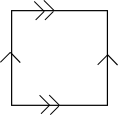
\includegraphics[scale=0.5]{./imagenes/toro.png}
  \end{figure}
  Se identifican los puntos
  \begin{gather*}
    (0,t) \sim (1,t), \quad t \in [0,1] \\
    (t,0) \sim (t,1), \quad t \in [0,1]
  \end{gather*}
  Existe un homeomorfismos entre el toro y el espacio \(S^1 \times S^1\)
  dado por la siguiente función \(f\):
  \begin{align*}
    f : T &\longrightarrow S^1 \times S^1 \\
    (a,b) &\longmapsto \left( \left( \cos (2 \pi a) , \sin (2 \pi a) \right), \left( \cos (2 \pi b) , \sin (2 \pi b) \right) \right)
  \end{align*}
  la cual es biyectiva, continua y independiente respecto al
  representante de clase de los elementos identificados del toro. Luego
  pensamos en el toro como el espacio producto \(S^1 \times S^1\). Por
  el Teorema \ref{thm:prop-prod} y el párrafo anterior
  \[
    \pi \left( T \right) = \pi \left( S^1 \times S^1 \right) = \pi (S^1)
    \times \pi (S^1)
  \]
  omitiendo el punto de origen puesto que este es un espacio
  arco-conexo.
\end{ejemplo}

Para el caso del co-producto, caracterizar alguna inclusion desde el
teorema anterior no resulta tan claro como la caracterizacion dada por
el teorema de \vank el cual se estudiara en la seccion \ref{sec:vank}.
Sin embargo lo anterior al menos implica las inclusiones
\[ \pi (X) < \pi (X \vee Y),\ \pi (Y) < \pi (X \vee Y)\]
diciéndonos que el grupo de \(\pi (X \vee Y)\) debe de ser compatible
con cualquiera de los grupos que conformen su wedge sum.

Nuestra meta ahora sera conocer teoremas mas generales que nos respeten
la estructura del (co)-producto para simplificar cálculos de grupos
fundamentales, lo cual sera el enfoque de la siguiente sección.
